\documentclass[12pt,a4paper]{article}
\usepackage{geometry}
\usepackage{slashbox}
\geometry{
	a4paper,
	total={170mm,257mm},
	left=20mm,
	right=20mm,
	top=20mm,
	bottom=20mm
}
\usepackage{graphicx}
\usepackage{pdfpages}
\usepackage{placeins}
\usepackage{float}

\usepackage{polski}
\usepackage[utf8]{inputenc}

\begin{document}
	
	\begin{titlepage}
		\newgeometry{top=5.5cm, bottom=3cm}
		
		\centering
		{\huge\bfseries Logika układów cyfrowych lab.\par}
		
		\vspace{0.5cm}
		Prowadzący: Mgr inż. Antoni Sterna (E02-38m, wtorek 17:05) \\
	
		\vspace{1.1cm}
		{\Large sprawozdanie 7 - 2017.11.28\par}
		\vfill
		
		{\large\bfseries Jakub Dorda 235013\par}
		{\large\bfseries Marcin Kotas 235098\par}
		
		\vspace{1cm}
		\today \\ \LaTeX
		
		\restoregeometry
	\end{titlepage}

	\newgeometry{top=1.5cm, bottom=1.5cm, left=20mm, right=20mm}

	\section{Wprowadzenie/cel ćwiczeń}
	
		Celem ćwiczeń było poznanie podstaw projektowania automatów w wariantach Moore'a i Mealy. Należało zaprojektować grafy w obu wariantach dla subtraktora szeregowego oraz komparatora szeregowego. Dodatkowo przeprowadzona została synteza strukturalna komparatora w wariancie Mealy w celu uruchomienia go na zestawie UNILOG.
		
		
	\section{Graf}
	
		\begin{itemize}
			\item Wejścia: \(Z = \{Z_0, Z_1\}\)\\
				
				\(Z_0\) - \\
				\(Z_1\) - 
				
			\item Stany wewnętrzne: \(Q =\{Q_0, Q_1, Q_2, Q_3\}\)
				
				\begin{minipage}{{.5\textwidth}}
					\centering
					\begin{tabular}{r|cc}
						&	\(q_1\)	&	\(q_0\)\\\hline
						\(Q_0\)	&	0	&	0	\\
						\(Q_1\)	&	0	&	1	\\
						\(Q_2\)	&	1	&	0	\\
						\(Q_3\)	&	1	&	1	\\
					\end{tabular}
				\end{minipage}%
				\begin{minipage}{{.5\textwidth}}	
					\(Q_0\) - \\
					\(Q_1\) - \\
					\(Q_2\) - \\
					\(Q_3\) - \\
				\end{minipage}
				
			\item Funkcja wyjść: \(Y=\{Y_0, Y_1\}\)
				
				\(Y_0\) - \\
				\(Y_1\) - 
		\end{itemize}
		
%		\begin{figure}[H]
%			\centering
%			\includegraphics[width=.25\textwidth]{schem/diag.png}
%			\\
%			\vspace{.1cm}
%			Graf 2 - subtraktor szeregowy w wersji Mealy
%		\end{figure}

		\section{Tabela prawdy i tablice Karnaugh:}
			\begin{table}[H]
			\begin{minipage}{.5\textwidth}
				\caption{Tabela Prawdy - funkcja przejść}
				\vspace{0.2cm}
				\centering
				\begin{tabular}{ccc|cc|cccc}
					\multicolumn{3}{c|}{\(t\)}	&	\multicolumn{2}{c|}{\(t+1\)} &&&\\
					\(q_1\)	&	\(q_0\)	&	\(Z\)	&	\(q_1\)	&	\(q_0\)	&	\(J_1\)	&	\(K_1\)	&	\(J_0\)	&	\(K_0\)	\\\hline
					0	&	0	&	0	&	0	&	1	&	0	&	-	&	1	&	-	\\
					0	&	0	&	1	&	1	&	0	&	1	&	-	&	0	&	-	\\
					0	&	1	&	0	&	0	&	0	&	0	&	-	&	-	&	1	\\
					0	&	1	&	1	&	1	&	1	&	1	&	-	&	-	&	0	\\\hline
					1	&	0	&	0	&	1	&	1	&	-	&	0	&	1	&	-	\\
					1	&	0	&	1	&	0	&	0	&	-	&	1	&	0	&	-	\\
					1	&	1	&	0	&	1	&	1	&	-	&	0	&	-	&	0	\\
					1	&	1	&	1	&	1	&	1	&	-	&	0	&	-	&	0	\\
				\end{tabular}
				\vspace{2cm}
			
				\caption{Tabela Prawdy - funkcja wyjść}
				\vspace{0.2cm}
				\centering
				\begin{tabular}{ccc|c}
					\(q_1\)	&	\(q_0\)	&	\(Z\)	&	\(Y\)	\\\hline
					0	&	0	&	0	&	0	\\
					0	&	0	&	1	&	0	\\
					0	&	1	&	0	&	1	\\
					0	&	1	&	1	&	0	\\\hline
					1	&	0	&	0	&	0	\\
					1	&	0	&	1	&	1	\\
					1	&	1	&	0	&	0	\\
					1	&	1	&	1	&	0	\\
				\end{tabular}
			\end{minipage}%
			\begin{minipage}{.5\textwidth}
				\caption{Tablica Karnaugh dla $J_1$}
				\vspace{0.2cm}
				\centering
				\begin{tabular}{c|c|c|c|c}
					\backslashbox{$Z$}{$q_1q_0$}	&	0	&	1	&	11	&	10	\\\hline
					"0	"	&	0	&	0	&	-	&	-	\\\hline
					"1	"	&	1	&	1	&	-	&	-	
				\end{tabular}
				
				\caption{Tablica Karnaugh dla $K_1$}
				\vspace{0.2cm}
				\centering
				\begin{tabular}{c|c|c|c|c}
					\backslashbox{$Z$}{$q_1q_0$}	&	0	&	1	&	11	&	10	\\\hline
					"0	"	&	-	&	-	&	0	&	0	\\\hline
					"1	"	&	-	&	-	&	0	&	1	
				\end{tabular}
			\vspace{1cm}
			
				\caption{Tablica Karnaugh dla $J_0$}
				\vspace{0.2cm}
				\centering
				\begin{tabular}{c|c|c|c|c}
					\backslashbox{$Z$}{$q_1q_0$}	&	0	&	1	&	11	&	10	\\\hline
					"0	"	&	1	&	-	&	-	&	1	\\\hline
					"1	"	&	0	&	-	&	-	&	0	
				\end{tabular}
				
				\caption{Tablica Karnaugh dla $K_0$}
				\vspace{0.2cm}
				\centering
				\begin{tabular}{c|c|c|c|c}
					\backslashbox{$Z$}{$q_1q_0$}	&	0	&	1	&	11	&	10	\\\hline
					"0	"	&	-	&	1	&	0	&	-	\\\hline
					"1	"	&	-	&	0	&	0	&	-	
				\end{tabular}
			\vspace{1cm}
			
				\caption{Tablica Karnaugh dla $Y$}
				\vspace{0.2cm}
				\centering
				\begin{tabular}{c|c|c|c|c}
					\backslashbox{$Z$}{$q_1q_0$}	&	0	&	1	&	11	&	10	\\\hline
					"0	"	&	0	&	1	&	0	&	0	\\\hline
					"1	"	&	0	&	0	&	0	&	1	
				\end{tabular}
			\end{minipage}
			\end{table}
		
		\subsection{Minimalizacje:}
		
		\vspace{1cm}
		\begin{minipage}{.5\textwidth}
			\centering
			\(J_1=Z\)\\
			\(J_0=\bar{Z}\)
			
		\end{minipage}%
		\begin{minipage}{.5\textwidth}
			\centering
			\(K_1	=Z\bar{q_0}	=\overline{\overline{Z\bar{q_0}}}	=\overline{\bar{Z}+q_0}\)\\
			\(K_0	=\bar{Z}\bar{q_1}	=\overline{\overline{\bar{Z}\bar{q_1}}}	=\overline{Z+q_1}\)
		\end{minipage}
		
		\vspace{.5cm}
		\begin{displaymath}
			Y = \bar{Z}\bar{q_1}q_0 + Zq_1\bar{q_0}	= \overline{\overline{\bar{Z}\bar{q_1}q_0 + Zq_1\bar{q_0}}}	=\overline{\overline{\bar{Z}\bar{q_1}q_0} \cdot \overline{Zq_1\bar{q_0}}}
		\end{displaymath}
	
		\newpage
		\subsection{Użyte wzory:}
			\begin{equation}
			\overline{a\cdot b}=\bar{a}+\bar{b}
			\end{equation}
			\begin{equation}
			\overline{a+b}=\bar{a}\cdot\bar{b}
			\end{equation}
		
		\subsection{Schemat układu:}
		
		\vspace{1.5cm}
%		\begin{center}
%			\makebox[\textwidth]{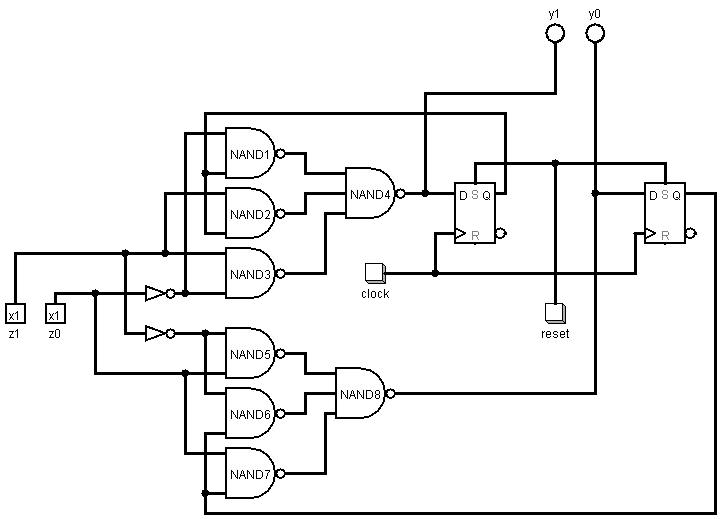
\includegraphics[width=\paperwidth - 30mm]{schem/circuitv2.png}}
%			Schemat 1 - komparator szeregowy w wersji Mealy
%		\end{center}

	\section{Wnioski/podsumowanie}
	
			W celu sprawdzenia poprawności działania komparatora należało przeprowadzić testy dla wszystkich możliwych kombinacji wejść oraz stanów. Za stan wejściowy przyjęto \(q_1=1, q_0 = 1\), więc przycisk reset należało podłączyć do wejść set przerzutników.
	
\end{document}